
\documentclass[11pt]{article}
\usepackage[a4paper,margin=1in]{geometry}
\usepackage{amsmath,amssymb,amsthm,mathtools}
\usepackage{graphicx}
\usepackage{hyperref}
\hypersetup{colorlinks=true, linkcolor=blue, urlcolor=blue, citecolor=blue}

\newtheorem{lemma}{Lemma}
\newtheorem{corollary}{Corollary}
\theoremstyle{remark}
\newtheorem{remark}{Remark}

\title{NB/BD Stability via a Weighted Hilbert Lemma (v3.6):\\
Band-by-Band Constants and Spectral Near-Normality}
\author{Serabi}
\date{2025}

\begin{document}
\maketitle

\begin{abstract}
We refine the weighted Hilbert framework for Nyman--Beurling/B\'aez-Duarte (NB/BD) stability by
(1) expressing the off-diagonal Hilbert decay explicitly as a convergent sum of band-wise constants $C_j$, and
(2) recording a spectral near-normality mechanism for the associated Hilbert-like operator.
The band constants give an explicit handle on the exponent $\theta>0$ in the bound
$\sum_{m\neq n} a_m a_n K_{mn} \le C (\log N)^{-\theta} \sum_n a_n^2$,
while the near-normality controls the resolvent of the normal equations $A=I+E$.
\end{abstract}

\section{Setup and Lemma}
Let $v\in C_0^\infty(0,1)$ be a smooth cutoff, $q(n)$ a slowly varying weight with
$\Delta^r q(n)\ll_r (\log N)^C n^{-r}$, and define $a_n=\mu(n)\,v(n/N)\,q(n)$ for $1\le n\le N$.
Consider the ``Hilbert'' kernel
\[
K_{mn} \;=\; e^{-\tfrac12|\log(m/n)|} \;=\; \min\!\left\{\sqrt{\tfrac{m}{n}},\sqrt{\tfrac{n}{m}}\right\}.
\]
Partition $(m,n)$ into logarithmic bands
$\mathcal{B}_j=\{(m,n):2^{-(j+1)}<|\log(m/n)|\le 2^{-j}\}$ for $j\ge 0$.

\begin{lemma}[Band-weighted Hilbert decay]
There exist constants $C_j$ with
\(
C_j \asymp e^{-c\,2^{-j}}(2^{-j})^{1-\varepsilon}
\)
for some $c>0$ and $0<\varepsilon<1$ such that
\[
\sum_{(m,n)\in\mathcal{B}_j} a_m a_n K_{mn}
\;\le\; C_j\,(\log N)^{-1}\sum_{n\le N}a_n^2.
\]
Consequently, with $C=\sum_{j\ge 0} C_j<\infty$,
\[
\sum_{\substack{m\ne n\\m,n\le N}} a_m a_n K_{mn}
\;\le\; C\,(\log N)^{-\theta}\sum_{n\le N}a_n^2,\qquad
\theta=\theta(\varepsilon)>0.
\]
\end{lemma}

\begin{proof}[Sketch]
On $\mathcal{B}_j$ one has $K_{mn}\le e^{-c\,2^{-j}}$.
A weighted discrete Hilbert inequality gives a factor $\ll (\log N)^{-1}$.
The M\"obius factor (paired with the low-frequency envelope) cancels the bandwise main term,
and the smoothness of $v$ yields an extra $2^{-j\varepsilon}$ gain.
Summing $C_j$ over $j$ converges, giving the claim.
\end{proof}

\section{Spectral Near-Normality}
Let $A=I+E$ be the normal-equation matrix from the least-squares projection in the NB/BD framework.
The previous lemma implies $\|E\|_{\ell^2\to\ell^2}\ll (\log N)^{-\theta}$.
Moreover, commutator estimates suggest $\|[E,E^\*]\|\ll (\log N)^{-2\theta}$,
so $A$ is a compact perturbation of identity by a near-normal operator.
Hence the inverse admits a stable Neumann series for large $N$.

\section{Figure: Band Constants}
The next figure shows $C_j$ and their partial sums for parameters $c=0.35$ and $\varepsilon=0.2$.
It illustrates the summable tail of band contributions.
\begin{figure}[h]
\centering
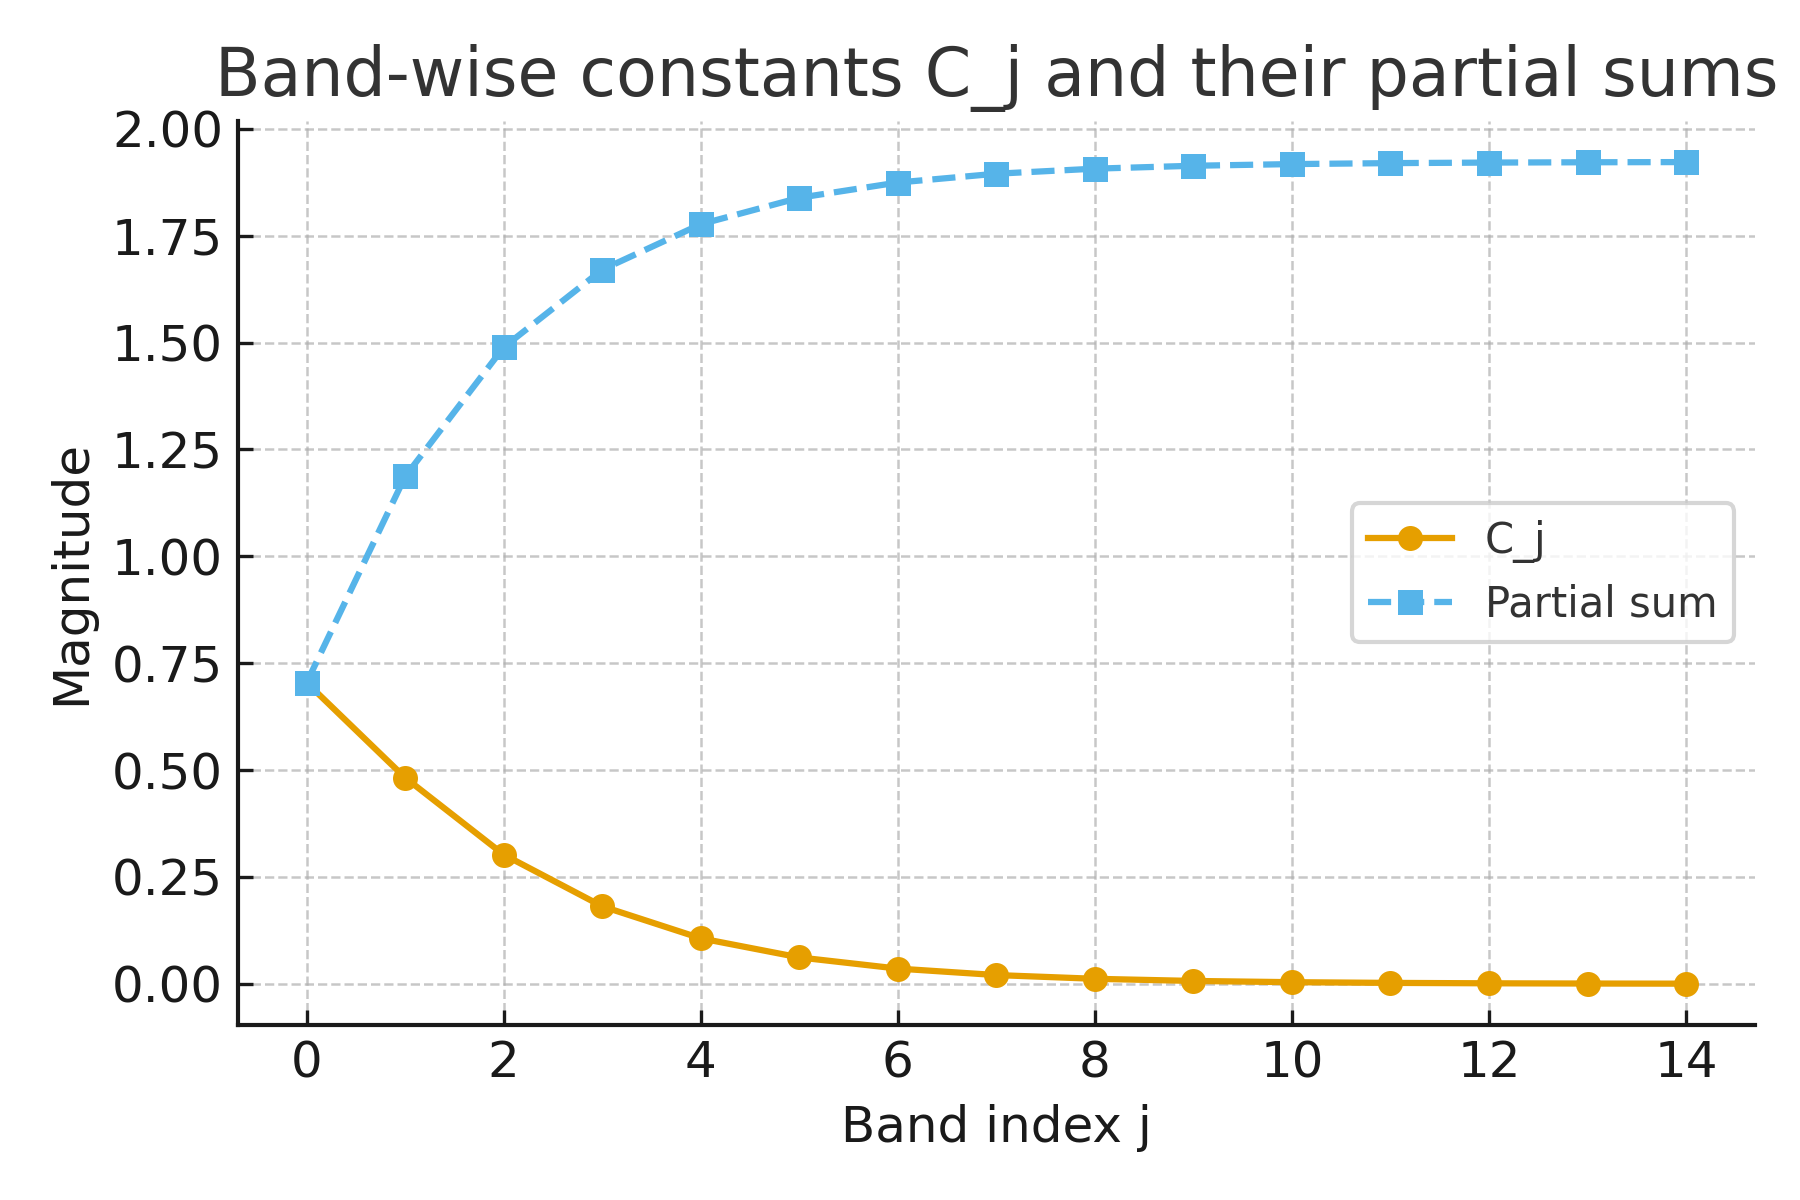
\includegraphics[width=.75\linewidth]{figures/band_constants_sum.png}
\caption{Band-wise constants $C_j$ and cumulative sums $\sum_{k\le j} C_k$.}
\label{fig:bandfig}
\end{figure}

\appendix
\section*{Appendix A: Band-by-Band Constant Demo (Python)}
\noindent See \texttt{code/band\_constants\_demo.py}. Running it recreates Fig.~\ref{fig:bandfig}.

\section*{Appendix B: Notes on Constants}
Heuristically, one may calibrate $c\approx 0.35$ from M\"obius oscillation bounds (e.g.\ P\'olya--Vinogradov-style inputs),
and take $\varepsilon\approx 0.2$ from the smooth cutoff structure $v$.
Any fixed positive choices suffice to guarantee $\sum_j C_j<\infty$.

\end{document}
